% !TeX program = xelatex
% !TeX encoding = UTF-8
\documentclass{MathModeling}
\usepackage{mwe,color,float}
\usepackage[linesnumbered,ruled]{algorithm2e}
\usepackage{setspace}
\usepackage{colortbl}
\usepackage{tablefootnote}
\everymath{\displaystyle}

\extrafloats{500}
\timu{\textbf{题目}}
\keyword{;号隔开}
\begin{document}
\setcounter{page}{1}
\pagestyle{fancy}
	\begin{abstract}
		最后,本文对所建立的模型进行中肯评价、提出改进措施,并对模型进行一定推广。
	\end{abstract}

	\section{问题的提出}
	\subsection{问题背景}
	作为一款单词猜谜游戏,Wordle每天都为玩家提供一个真正的英语单词作为谜题,现已推出60多种语言版本,本文以英文版本为例。其玩法为:玩家在6次或更少次数内猜出一个5个字母的单词以解决谜题。在此过程中,玩家每一次进行的猜测必须为真实存在的单词,提交后系统将对单词进行检测,若该位置显示为绿色则代表谜底单词含有该字母,且其位置正确;若为黄色则代表该字母存在但所在位置错误;若为灰色则谜底中不包含此字母。玩家可选择“常规模式”及“困难模式”进行挑战,其中在“困难模式”下玩家若找到谜底中包含的字母,即显示绿色及黄色砖块,在其后的猜测的单词中必须包含这些字母。Wordle官方统计了在Twitter上分享的每一天玩家通关所需次数。游戏两种模式玩法见\textcolor{blue}{\cref{fig:简单模式游戏}}及\textcolor{blue}{\cref{fig:困难模式游戏}}。
	\begin{figure}[H]
		\centering
		\begin{minipage}{0.48\linewidth}
			\centering
			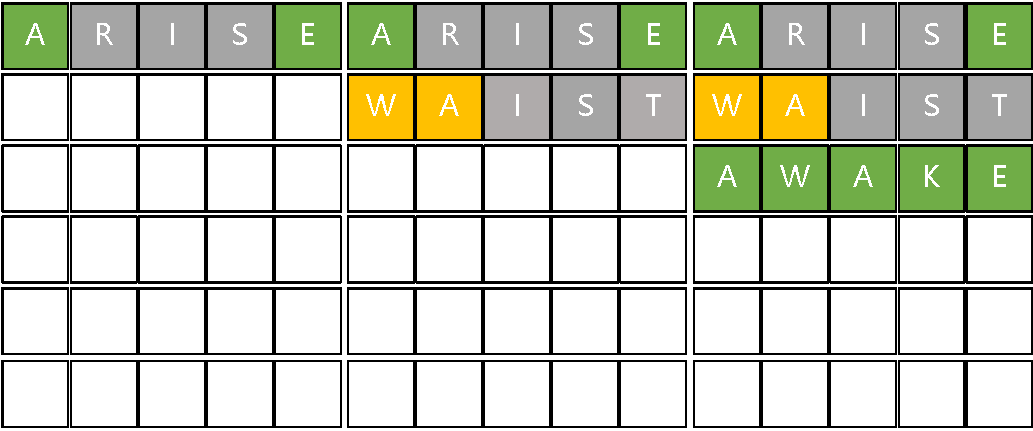
\includegraphics[width=0.96\linewidth]{简单模式图.pdf}
			\caption{常规模式}
			\label{fig:简单模式游戏}
		\end{minipage}
		%\qquad
		\begin{minipage}{0.48\linewidth}
			\centering
			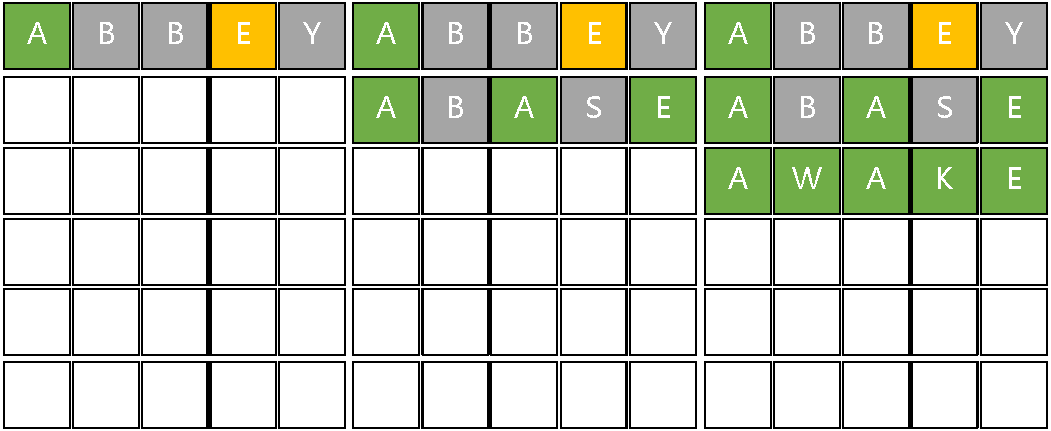
\includegraphics[width=0.96\linewidth]{困难模式图.pdf}
			\caption{困难模式}
			\label{fig:困难模式游戏}
		\end{minipage}
	\end{figure}

	\subsection{问题要求}
	\begin{itemize}
		\item \textbf{问题一}:官方所提供报告的结果每天数量均存在差异,建立一个模型以解释该差别并预测2023年5月15日报告结果的数量区间。分析单词属性对于困难模式得分比例是否存在影响,并解释其原因。
		\item \textbf{问题二}:建立模型预测未来谜底单词的报告结果相关百分比,说明该模型预测有哪些不确定性,并以单词“EERIE”的预测为例分析模型效果。
		\item \textbf{问题三}:建立一个依据单词难度分类的模型,并对谜底单词分类。确定各类别中谜底单词属性及单词“EERIE”的难度并分析该模型的准确性。
		\item \textbf{问题四}:进一步分析数据集中其他有趣的特征。
		\item \textbf{问题五}:写一封信函向《纽约时报》的谜底编辑总结分析结果。
	\end{itemize}

	\section{问题的分析}
	\subsection{问题的整体分析}
	该题是一个以热门游戏Wordle为背景的数据分析,自然语言处理,预测类问题。

	\textbf{从分析目的看},本题需要以单词的属性进行分析,筛选出影响玩家得分比例的主要因素,确定各分类相关联的给定单词的属性并总结,量化结果。同时还须对玩家的得分结果进行预测与研究,为《纽约时报》的谜题编辑提供参考,以进一步优化Wordle游戏。因此本题主要需要完成以下几方面的任务:{\heiti 其一},分析每日报告结果数量的变化情况;{\heiti 其二},确定单词属性与困难模式游玩得分的关系;{\heiti 其三},预测特定单词玩家尝试次数的百分比;{\heiti 其四},分析单词属性与单词难度的关联性;{\heiti 其五},进一步探讨数据集具有的有趣特征;{\heiti 其五}:写一封信函向《纽约时报》的谜底编辑总结分析结果。

	\textbf{从数据来源、特征看},本题的数据来源于2022年2月7日至2022年12月31日Twitter玩家分享游戏结果,数据包括“日期”“编号”“谜底单词”“答案提交数”“困难模式参与数”“1$\sim$7次尝试分布比例”。但未提高对数据的分析能力,提升预测效果,挖掘更多有效信息,我们将对2023年数据进行爬取,构造与附件数据一致的数据,两者综合进行分析。同时我们发现数据具有高维,量纲不一致等特点,且数据体量较大,因此,本题相对复杂,需对数据进行一定的预处理,以便于后续分析。

	\textbf{从模型的选择看},本题数据的时间跨度大,维度较高,且需预测未来的报告数和相关百分比的分布、基于单词难度对单词进行分类。因此本文选择XGboost回归模型、随机森林回归模型进行预测分析,同时利用K-means模型对单词进行分类,在该分类基础上建立数据标签,并采用SVM模型对单词“EERIE”进行预测。

	\textbf{从编程软件的选择看},本题为数据分析类,需要进行数据预处理、数据分析、数据可视化,并依据各设问建立不同类别的模型,因此我们选择Python Jupyter Notebook对问题进行求解,其交互式的编程范式及轻量化,方便且高效。
	
	\subsection{问题一的分析}
	问题一的核心目的有以下几点:{\heiti 其一},\textbf{对报告数据进行预处理,去伪存真};{\heiti 其二},\textbf{研究每日结果数据的变化};{\heiti 其三},预测2023年5月15日报告结果数量,并建立一个合理区间;{\heiti 其四},\textbf{研究分析单词属性与困难模式得分的关系}。对于给定的数据集,我们发现部分数据在正确性,完整度性等方面存在一定缺陷,因此我们须对数据集进行预处理。由于附数据体量较大,因此我们将将总人数,选择困难模式人数及其变化率数据可视化,直观分析变化规律并建立普适性预测模型。同时我们还考虑到游戏人数数据等不符合正态分布,因此我们放弃线性回归而选择XGBoost模型进行回归预测。此外我们对单词进行属性分析,利用Python自然语言处理nltk库,建立单词的属性模型,并绘制皮尔逊相关系数热力图分析其中的关系。

	\subsection{问题二的分析}

	\subsection{问题三的分析}
	问题三的核心目的在于\textbf{根据单词难度对单词进行分类}。因此我们结合问题一所构造的特征及相关指标,对样本数据进行K-means聚类分析,并结合肘部法则选择合适的$k$值,绘制PCA降维聚类结果散点图,观察聚类效果。在对样本数据进行分类后,将难度定义为词汇的分类标准,采用SVM模型对分类的结果进行更详细的定性及定量分析。最后对单词“EERIE”进行分析,确定其难度。此外我们还需对模型进行合理性分析,绘制分类报告、混淆矩阵热力图、ROCAUC曲线、分类预测结构,从而更好地探讨其效果。

	\subsection{问题四的分析}
	
	\subsection{问题五的分析}
	
	\section{模型的假设}
	\begin{itemize}
		\item \textbf{假设一}:假设个体在单词认知能力上差异较小。
		\item \textbf{假设二}:假设《纽约时报》每一天的谜底单词均随机抽取,不受人为等因素干扰。
		\item \textbf{假设三}:假设每日参与游戏人数不会出现较为明显的波动,在一定范围内稳定。
		\item \textbf{假设四}:假设若玩家在六次及以内未能成功猜出谜底单词,则游戏失败。并将游戏失败的玩家视作进行7次尝试。
	\end{itemize}
	\section{符号说明}
	\begin{center}
		\begin{tabularx}{0.7\textwidth}{c@{\hspace{1pc}}|@{\hspace{2pc}}X}
			\Xhline{0.08em}
			符号 & \multicolumn{1}{c}{符号说明}\\
			\Xhline{0.05em}
			$\mu$ & 样本平均数 \\
			$\sigma$ & 样本标准差 \\
			$x_{\mathrm{standard}}$ & 经过标准化后的数据\\
			$R\left(x\right)_{m\times n}$ & 经过某项处理后的数据特征集\\
			$\hat{y}$ & 预测值\\
			$L^{\left(t\right)}$ & 目标函数\\
			$\omega$ & 权重\\
			\Xhline{0.08em}
		\end{tabularx}
	\end{center}

	\textbf{注:}这里并未列出部分变量,这是由于它们在不同小节处有不同的含义,因此我们会在每一节中详细讨论它们。
	\section{模型的建立与求解}
	对于本题,本文模型的建立与求解部分主要分为数据的准备,模型的建立、求解、结果分析。
	\begin{itemize}
		\item \textbf{数据的准备}:爬取2023年数据,提高模型分析数据的准确性。并对于构建的新数据集进行预处理,方便后续模型的建立;
		\item \textbf{模型的建立、求解、结果分析}:对于给定的数据集及爬取的新数据集,本文依据其特点,建立合适的回归、聚类、分类模型,并进行多种数据可视化,分析模型效果。
	\end{itemize}

	\subsection{数据的准备}
	本部分我们需要爬取2023年的数据,以提高模型分析数据的准确性。同时还需要对数据集进行一定的预处理,对错误值进行修正,以便后续模型的建立。本部分我们所利用的数据收集网站见\textcolor{blue}{\cref{tab:数据来源}}。

\begin{table}[H]
	\centering
	\caption{数据来源}
	\scalebox{0.95}{
	  \begin{tabular}{cc}
	  \toprule
	  \textbf{网址} & \textbf{描述} \\
	  \midrule
	  \url{https://m.stockq.org/life/wordle-history.php\#all} & Wordle每日答案统计 \\
	  \url{https://twitter.com/WordleStats} & Wordle每日报告结果 \\
	  \bottomrule
	  \end{tabular}}
	\label{tab:数据来源}
\end{table}
	\subsubsection{2023年数据爬取}
观察原数据集,其统计的为2022年2月7日至2022年12月31日的情况,而缺少2023年数据,且问题需要预测2023年5月15日数据,因此为提高模型精度,我们将对2023年数据进行爬取,并与原数据集进行合并,使得在游戏编号、时间方面连续。新数据集读者可在附件中查阅。其中部分数据见\textcolor{blue}{\cref{tab:2023年部分数据}},新数据集截止至2023年4月25日。
\begin{table}[H]
	\centering
	\caption{2023年部分数据}
	\scalebox{0.95}{
	  \begin{tabular}{ccccc}
	  \toprule
	  Date  & Contest number & Word  & Number of reported results & Number in hard mode \\
	  \midrule
	  2023/1/1 & 561   & whine & 22072 & 2132 \\
	  2023/1/2 & 562   & skirt & 22252 & 2094 \\
	  2023/1/3 & 563   & antic & 22018 & 2072 \\
	  2023/1/4 & 564   & layer & 22394 & 2207 \\
	  2023/1/5 & 565   & sleek & 22283 & 2078 \\
	  \bottomrule
	  \end{tabular}}
	\label{tab:2023年部分数据}
\end{table}
  
	\subsubsection{异常单词的修正}
	根据Wordle游戏规则,每日谜底单词均为5个字母长度,因此我们对原数据集所有单词进行分析,筛选出字母数不为5个的单词,并依据Wordle游戏每日单词统计的数据与游戏编号进行比对,将上述错误单词替换为正确单词,更换结果见\textcolor{blue}{\cref{tab:单词修正}}。
\begin{table}[H]
	\centering
	\caption{单词修正}
	\scalebox{0.95}{
	  \begin{tabular}{ccc}
	  \toprule
	  \textbf{游戏编号} & \textbf{异常单词} & \textbf{替换单词} \\
	  \midrule
	  207   & favor \textcolor{blue}{\tablefootnote{该单词错误原因是在表格数据中其后有一空格,该空格会影响后续问题的解决。}}  & favor \\
	  314   & tash  & trash \\
	  525   & clen  & clean \\
	  545   & rprobe & probe \\
	  \bottomrule
	  \end{tabular}}
	\label{tab:单词修正}
\end{table}
  
	\subsubsection{人数异常值}
	为了更好地初步发现异常值,我们绘制出每日游戏报告结果总人数及选择困难游戏模式人数变化图,如\textcolor{blue}{\cref{fig:总人数及选择困难游戏模式人数变化图}}。观察该图,我们可以发现,2022年11月30日总人数突然减少明显,但其对应的选择困难人数并未有明显变化,且两者数据相近。因此,这里我们定义其为离群点,其明显不符合发展变化规律,对其的处理,我们将再下文展开分析。
	\begin{figure}[H]
		\centering
		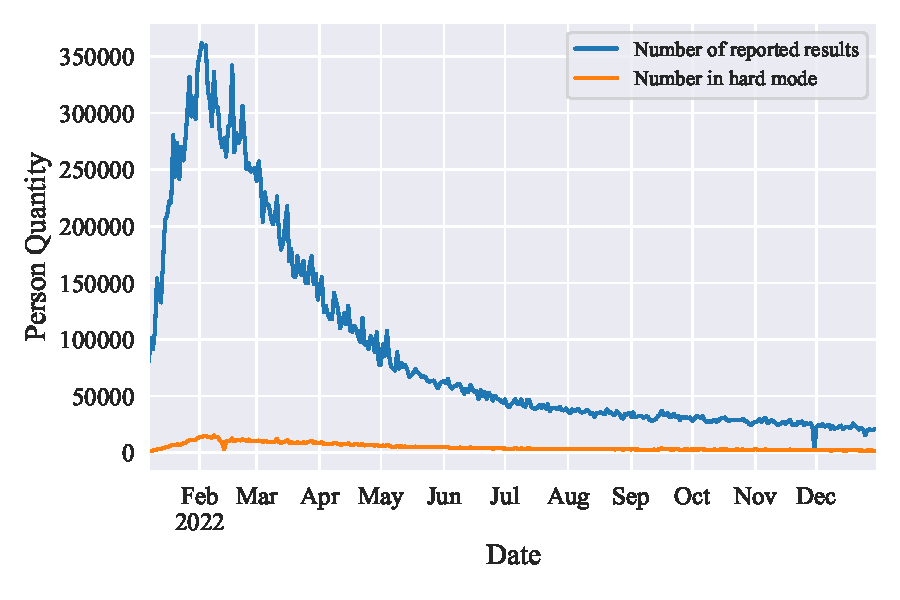
\includegraphics[width=0.55\textwidth]{报告结果每日变化.pdf}
		\caption{总人数及选择困难游戏模式人数日变化}
		\label{fig:总人数及选择困难游戏模式人数变化图}
	\end{figure}

	同时我们还计算出每日选择困难人数占总人数的比例,绘制出每日选择困难模式人数频率变化及变化率图示,见\textcolor{blue}{\cref{fig:每日选择困难模式人数频率变化}}及\textcolor{blue}{\cref{fig:每日选择困难模式人数频率变化率}}。
	\begin{figure}[H]
		\centering
		\begin{minipage}{0.48\linewidth}
			\centering
			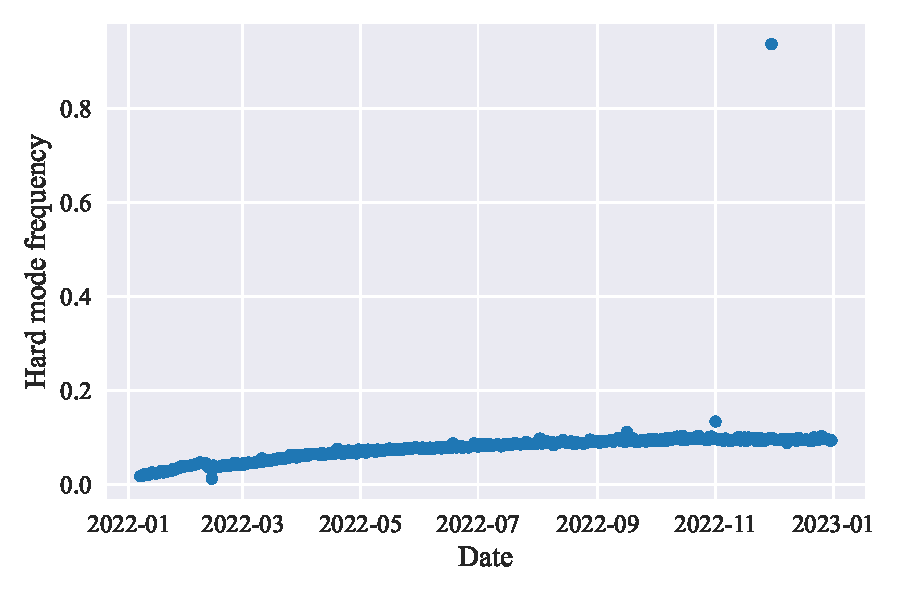
\includegraphics[width=0.96\linewidth]{每日选择困难模式人数频率变化.pdf}
			\caption{每日选择困难模式人数频率变化}
			\label{fig:每日选择困难模式人数频率变化}
		\end{minipage}
		%\qquad
		\begin{minipage}{0.48\linewidth}
			\centering
			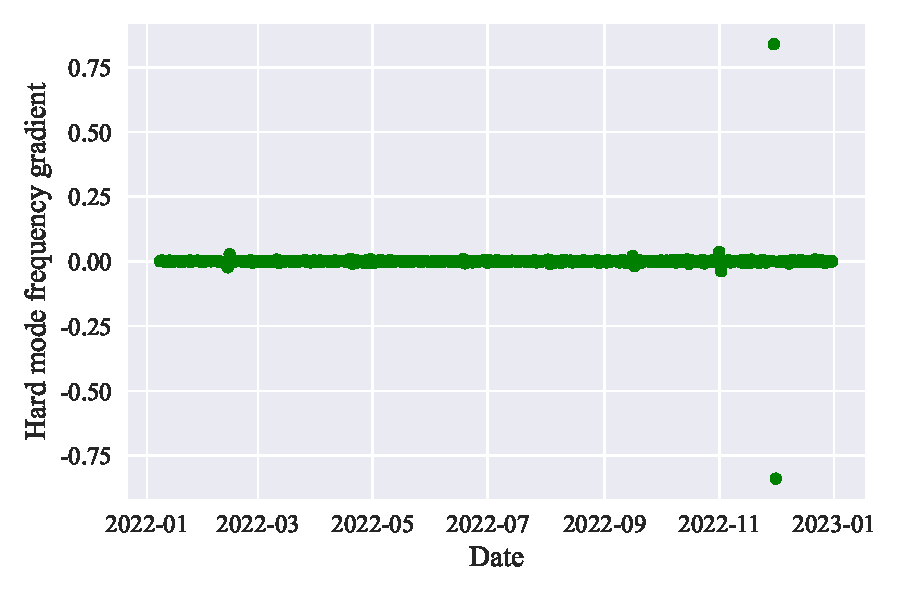
\includegraphics[width=0.96\linewidth]{每日选择困难模式人数频率变化率.pdf}
			\caption{每日选择困难模式人数频率变化率}
			\label{fig:每日选择困难模式人数频率变化率}
		\end{minipage}
	\end{figure}
	通过观察上述两幅图,我们可以清晰发现异常值,但也存在部分图示上难以鉴别的离群点,因此这里我们设定变化率阈值为$0.02$,若每日变化率绝对值超过该阈值,且在相邻两天内变化率绝对值超过该阈值,则定义其为离群点,对其进行处理。这是由与若某一天突变严重,会引起当天与后一天变化率均会超过阈值,而真正地异常值应为首次超过的那一天。但异常值为总人数还是选择困难游戏人数,我们还需要结合改日前后几天数据记性判断。通过筛选,我们得到异常数据,见\textcolor{blue}{\cref{tab:异常数据}}。
\begin{table}[H]
	\centering
	\caption{异常数据分析}
	\scalebox{0.95}{
	  \begin{tabular}{cccccc}
	  \toprule
	  \textbf{游戏编号} & \textbf{当日单词} & \textbf{游戏总人数} & \textbf{选择困难模式人数} & \textbf{选择困难人数变化率} & \textbf{异常值} \\
	  \midrule
	  239   & robin & 277471 & 3249  & -0.022787  & 3249 \\
	  240   & ultra & 261521 & 10343 & 0.027840  & 无 \\
	  500   & piney & 27502 & 3667  & 0.036272  & 3667 \\
	  501   & inept & 27670 & 2640  & -0.037926  & 无 \\
	  529   & study & 2569  & 2405  & 0.838601  & 2569 \\
	  530   & eject & 22628 & 2200  & -0.838937  & 无 \\
	  \bottomrule
	  \end{tabular}}
	\label{tab:异常数据}
\end{table}

	\subsubsection{百分比异常值}
	根据对原数据集中尝试次数百分比的理解,其7次累计和应为$1$,因此我们计算数据中玩家尝试次数百分比的累计和,我们发现,除游戏编号为$281$的数据累计百分比为$126\,\%$,其余数据均在$\left(100\pm2\right)\,\%$的范围内,因此我们有理由认为该天存在统计误差,并记为异常值。
	\subsubsection{异常值处理}
对于异常值的处理,为了尽可能保留数据信息,我们采用拉格朗日插值法,对上述异常数据进行修正。
拉格朗日插值法(Lagrange's Interpolation)是一种多项式插值的方法。对于给定的$n+1$个坐标不同的点,其可以给出一个恰好经过这$n+1$个点的多项式函数。拉格朗日基本多项式(插值基函数)如下
\begin{equation}
	l_{j}\left(x\right)=\prod_{i=0,i\neq j}^{n}\frac{x-x_{i}}{x_{j}-x_{i}},j=0,1,\cdots,n
\end{equation}
则拉格朗日插值多项式为
\begin{equation}
	L\left(x\right)=\sum_{j=0}^{n}y_{j}l_{j}\left(x\right)
\end{equation}
此多项式经过给定的$n+1$个点。

经过上述处理后,我们对异常值进行了修正,得到了新的数据,见\textcolor{blue}{\cref{tab:异常值修正后数据1}}及\textcolor{blue}{\cref{tab:异常值修正后数据2}}。
\begin{table}[H]
	\centering
	\caption{人数异常值修正}
	\scalebox{0.95}{
	  \begin{tabular}{cccccc}
	  \toprule
	  \textbf{游戏编号} & \textbf{当日单词} & \textbf{游戏总人数} & \textbf{选择困难模式人数} & \textbf{异常值} & \textbf{修正值} \\
	  \midrule
	  239   & robin & 277471 & 3249  & 3249  & 9249 \\
	  500   & piney & 27502 & 3667  & 3667  & 2667 \\
	  529   & study & 2569  & 2405  & 2569  & 25569 \\
	  \bottomrule
	  \end{tabular}}
	\label{tab:异常值修正后数据1}
\end{table}
\begin{table}[H]
	\centering
	\caption{百分比异常值修正}
	\scalebox{0.88}{
	  \begin{tabular}{cccccccccc}
	  \toprule
	  \textbf{类} & \textbf{游戏编号} & \textbf{1 try} & \textbf{2 tries} & \textbf{3 tries} & \textbf{4 tries} & \textbf{5 tries} & \textbf{6 tries} & \textbf{X} & \textbf{百分比和} \\
	  \midrule
	  异常值   & 281   & 1     & 2     & 18    & 44    & 26    & 26    & 9     & 126 \\
	  修正值   & 281   & 1     & 2     & 18    & 44    & 26    & 9     & 1     & 101 \\
	  \bottomrule
	  \end{tabular}}
	\label{tab:异常值修正后数据2}
\end{table}
	\subsection{问题一模型的建立与求解}
	对于该问题,我们需要完成以下几点任务:
	\begin{itemize}
		\item 分析每日报告结果变化情况,并建立模型来解释这种变化;
		\item 利用上述模型对2023年5月15日的报告结果进行预测,并设定置信区间;
		\item 分析单词属性是否会影响困难模式下玩家尝试次数的比例,并解释原因。
	\end{itemize}
	因此,该部分我们围绕上述任务进行分析、解决。
	\subsubsection{每日报告结果分析}
	根据对数据集进行观察,我们发现游戏编号是按顺序进行连续编号的,因此游戏编号可以看作是对数据集无影响的序列。我们按游戏编号将报告结果绘制为散点图,并绘制出数据变化的整体趋势,如\textcolor{blue}{\cref{fig:每日报告结果变化趋势}}所示。
	\begin{figure}[H]
		\centering
		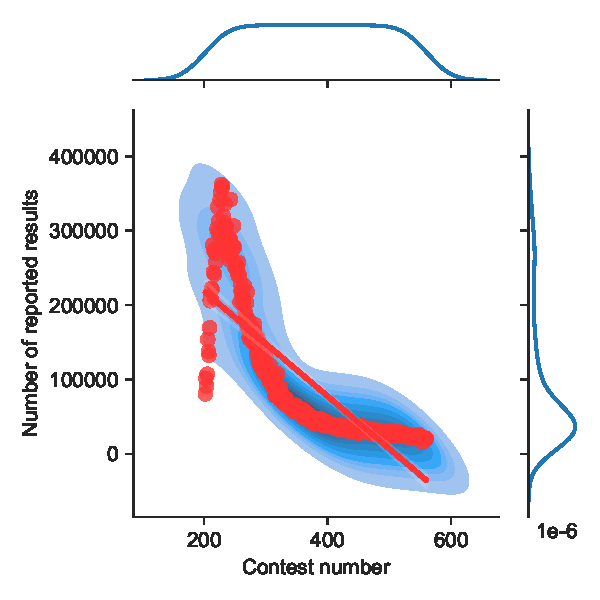
\includegraphics[width=0.5\textwidth]{核密度估计值.pdf}
		\caption{每日报告结果变化趋势}
		\label{fig:每日报告结果变化趋势}
	\end{figure}
	观察该图,我们可以发现报告结果呈现了先增加后减小的趋势,最后逐渐趋近于稳定。其在一定程度上反映了游戏玩家的人数变化规律。考虑到游戏存在生命周期,我们认为报告结果的现象与游戏生命周期存在关系。因此考虑到游戏或信息的传播一般会经历增长、成熟、衰退和稳定的时期。报告结果是当天玩与分享Twitter的Wordle玩家的数量。同时我们认为推文的数量主要受玩家数量的影响,同时更多的推文也将吸引更多的玩家。当普通的Twitter用户看到一条关于这款游戏的推文时,他们将有$\alpha$的概率成为一位新的Wordle玩家。当一位玩家试玩该游戏后,他将会有$\beta$的概率发送一条推文,成为一位普通玩家。曾时试玩的玩家有$\gamma$的概率返回游戏,同时玩家将在多次比赛后有$\sigma$的概率第二天不再游戏。因此我们有理由认为报告结果的数量不仅仅与表层的时间序列有关,而有更深次的内在联系。因此这里我们将不考虑时间序列模型进行预测。同时,考虑线性回归模型,此时我们需要检验该数据是否符合正态分布,因此我们绘制随机变量直方图、概率密度图以及Q-Q图(Quantile-Quantile Plot),如\textcolor{blue}{\cref{fig:正态分布分析}}所示。
	\begin{figure}[H]
		\centering
		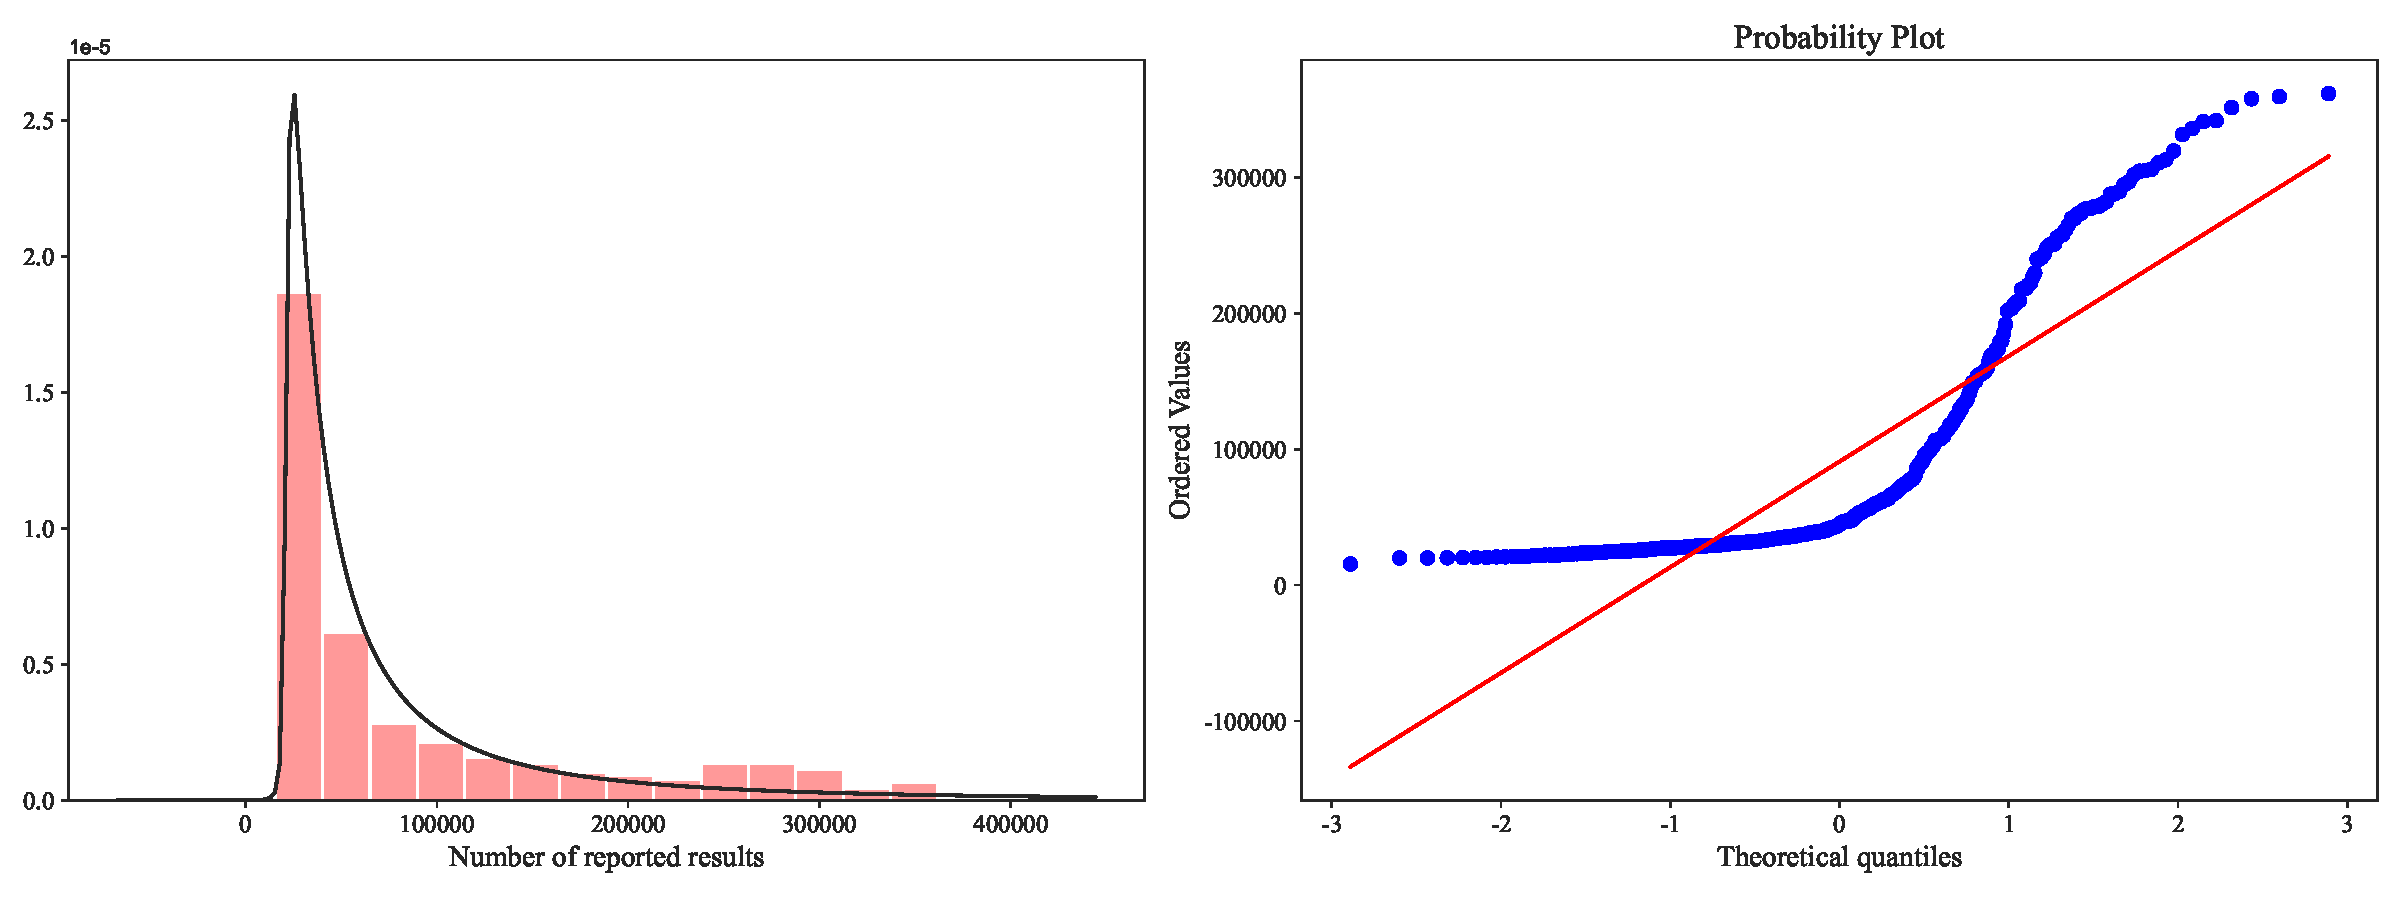
\includegraphics[width=0.95\textwidth]{正态分布分析.pdf}
		\caption{正态分布分析}
		\label{fig:正态分布分析}
	\end{figure}
dgy分析

	因此我们有理由认为对于该数据集,进行线性回归分析可能会在一定程度上得到较优效果,但这并不是在数据集集中部分的效果,极有可能会对未来的预测产生较大误差,因此我们考虑建立极端梯度提升(eXtreme Gradient Boosting,XGBoost)模型,首先对每日报告总人数进行预测,再对选择困难模式人数进行预测分析。
	XGBoost算法是一种基于树模型的优化模型,该算法通过多次迭代,生成一个新的树模型用于优化前一个树模型,随着迭代次数的增多,该模型的预测精度也会相应提高\textcolor{blue}{\cite{pxgboost1}}。

		记通过数据处理后的数据集特征为$R\left(x_{ij}\right)_{m\times n}$,表示其包含$m$天的游戏情况,$n$个特征,在训练中形成的CART树的集合记为$F=\left\{f\left(x\right)=w_{q\left(x\right)},q:\mathbf{R}^n\to T,w\in \mathbf{R}^T\right\}$,其中$q$为树模型的叶节点决策规划,$T$为某一树模型叶节点数量,$w$为叶节点对应的得分\textcolor{blue}{\cite{pxgboost2}}。对于预测的$y$值,其计算公式为
		\begin{equation}
			\hat{y}=\varphi \left( x_i \right) =\sum\limits_{k=1}^K{f_k\left( x_i \right)} \label{fXGBoostypre}
		\end{equation}
	
		XGBoost算法在每一次迭代过程中会保存前面所学习的模型,会将这些模型加入到新一轮迭代过程中,因此我们记第$i$个模型为预测结果为
		\begin{equation}
			\hat{y}_{i}^{\left(t\right)}=\hat{y}_{i}^{\left(t-1\right)}+f_t\left(x_i\right) \label{fXGBoostyprei}
		\end{equation}
		
		XGBoost算法的目标函数计算公式如下
		\begin{equation}
			L^{\left(t\right)}=\sum\limits_{i=1}^{n}l\left(y_i,\hat{y}_{i}^{\left(t-1\right)}+f_t\left(x_i\right)\right)+\gamma T+\frac{1}{2}\lambda\sum\limits_{j=1}^T{w_j^2}+\mathrm{const} \label{fXGBoostL}
		\end{equation}
		上述公式中,$l$为模型误差损失,描述在该模型下预测值与实际值之间的出差异损失,$\Omega$为模型叶节点的正则项惩罚系数,$\gamma$与$\lambda$为模型的超参数\textcolor{blue}{\cite{pxgboost2}}。
		
		通常情况下,我们难以用枚举法得到在模型中所训练出来的树结构,因此这里采用贪婪算法,从单叶子节点开始,通过迭代方法,将其加入到树结构中,从而得到最优解,其计算公式\textcolor{blue}{\cite{pxgboost3}}如下
		\begin{equation}
			\mathcal{L}_{split}=\frac{1}{2}\left[\frac{\left(\sum_{i\in I_L}g_i\right)^2}{\sum_{i\in I_L}h_i+\lambda}+\frac{\left(\sum_{i\in I_R}g_i\right)^2}{\sum_{i\in I_R}h_i+\lambda}-\frac{\left(\sum_{i\in I}g_i\right)^2}{\sum_{i\in I}h_i+\lambda}\right]-\gamma \label{fXGBoostLsplit}
		\end{equation}
		其中$I_j=\left\{i|q\left(x_i\right)=j\right\}$为叶节点$j$上的样本集合\textcolor{blue}{\cite{pxgboost2}},且有
		\begin{equation}
			g_i=\partial_{\hat{y}^{\left(t-1\right)}}l\left(y_i,\hat{y}_i^{\left(t-1\right)}\right)
		\end{equation}
		\begin{equation}
			h_i=\partial_{\hat{y}^{\left(t-1\right)}}^2l\left(y_i,\hat{y}_i^{\left(t-1\right)}\right)
		\end{equation}

	\subsubsection{预测2023年5月15日数据}
	依据上述分析,我们首先以报告结果总人数为预测目标,再以报告选择困难模式玩家人数为预测目标对数据集进行训练以及测试\textcolor{blue}{\footnote{对于报告结果总人数预测,我们仅传入游戏编号序列作为自变量;对于报告结果选择困难模式人数预测,我们传入游戏编号及总人数序列作为自变量}}。划分训练集及测试集比例为$9:1$,通过XGBoost算法对训练集进行训练,同时在测试集上进行评估。我们得到训练测试拟合图,见\textcolor{blue}{\cref{fig:XGBoost预测结果总人数}}及\textcolor{blue}{\cref{fig:XGBoost预测结果困难人数}}。
	\begin{figure}[H]
		\centering
		\begin{minipage}{0.48\linewidth}
			\centering
			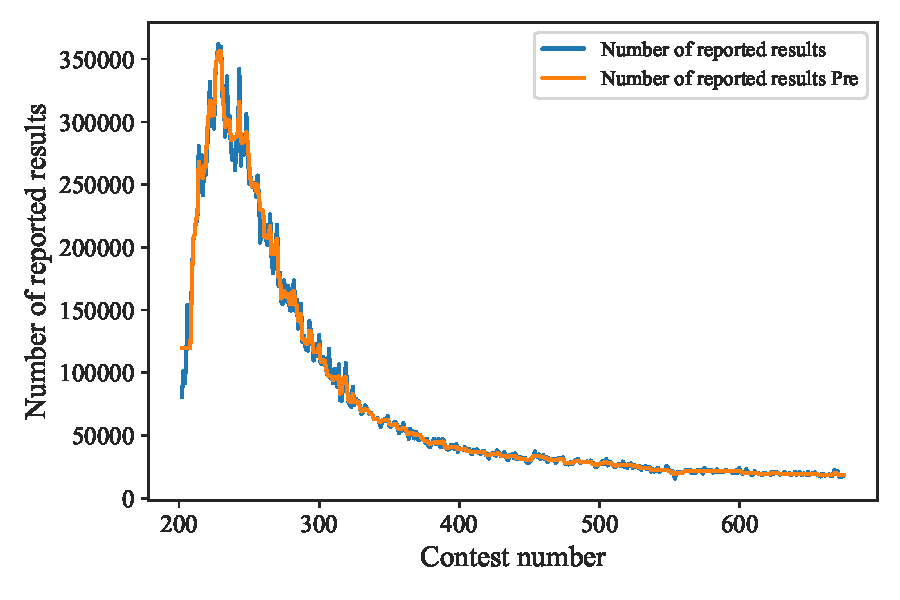
\includegraphics[width=0.98\linewidth]{XGBoost预测结果(总人数).pdf}
			\caption{XGBoost预测结果-总人数}
			\label{fig:XGBoost预测结果总人数}
		\end{minipage}
		%\qquad
		\begin{minipage}{0.48\linewidth}
			\centering
			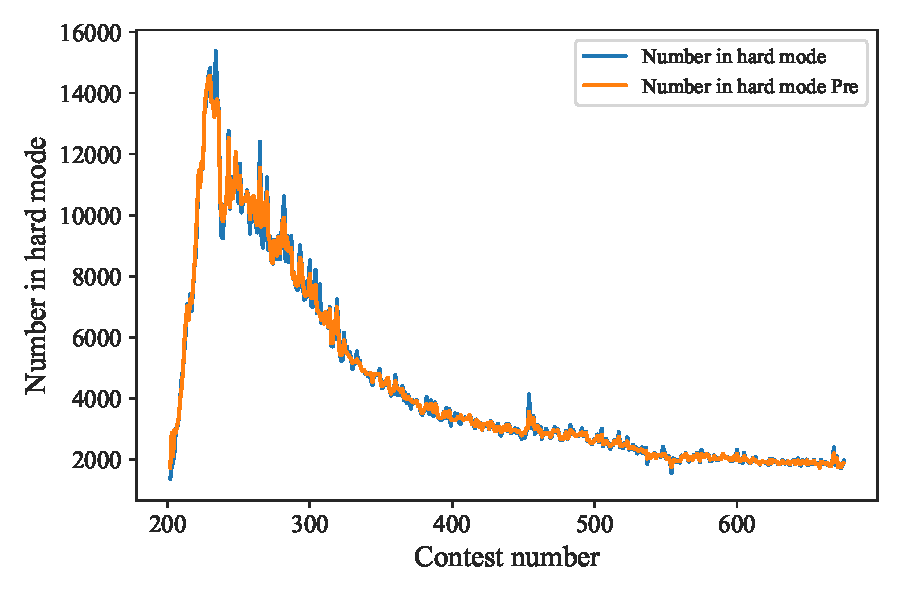
\includegraphics[width=0.98\linewidth]{XGBoost预测结果(困难人数).pdf}
			\caption{XGBoost预测结果-困难人数}
			\label{fig:XGBoost预测结果困难人数}
		\end{minipage}
	\end{figure}
	同时我们还绘制上述两个模型的预测误差图,见\textcolor{blue}{\cref{fig:XGBoost预测误差总人数}}及\textcolor{blue}{\cref{fig:XGBoost预测误差困难人数}}。
	\begin{figure}[H]
		\centering
		\begin{minipage}{0.48\linewidth}
			\centering
			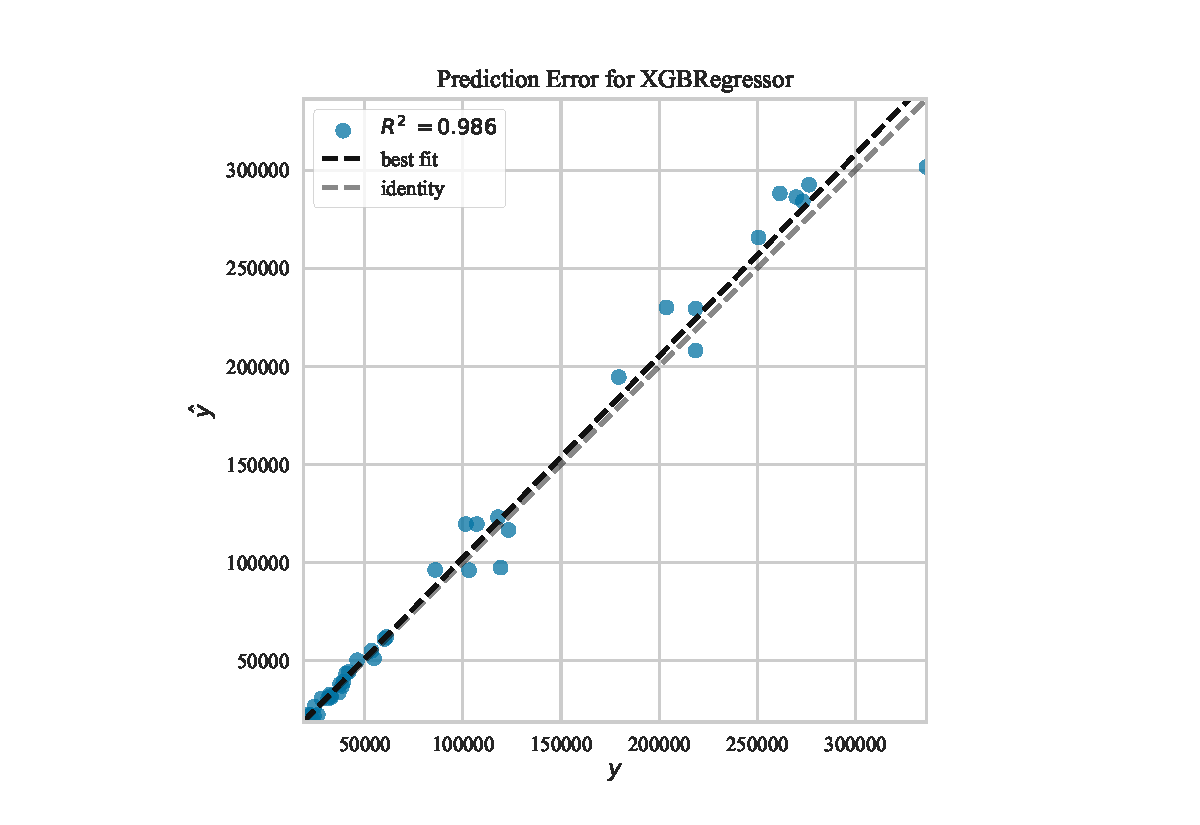
\includegraphics[width=1.0\linewidth]{XGBoost预测误差(总人数).pdf}
			\caption{XGBoost预测误差-总人数}
			\label{fig:XGBoost预测误差总人数}
		\end{minipage}
		%\qquad
		\begin{minipage}{0.48\linewidth}
			\centering
			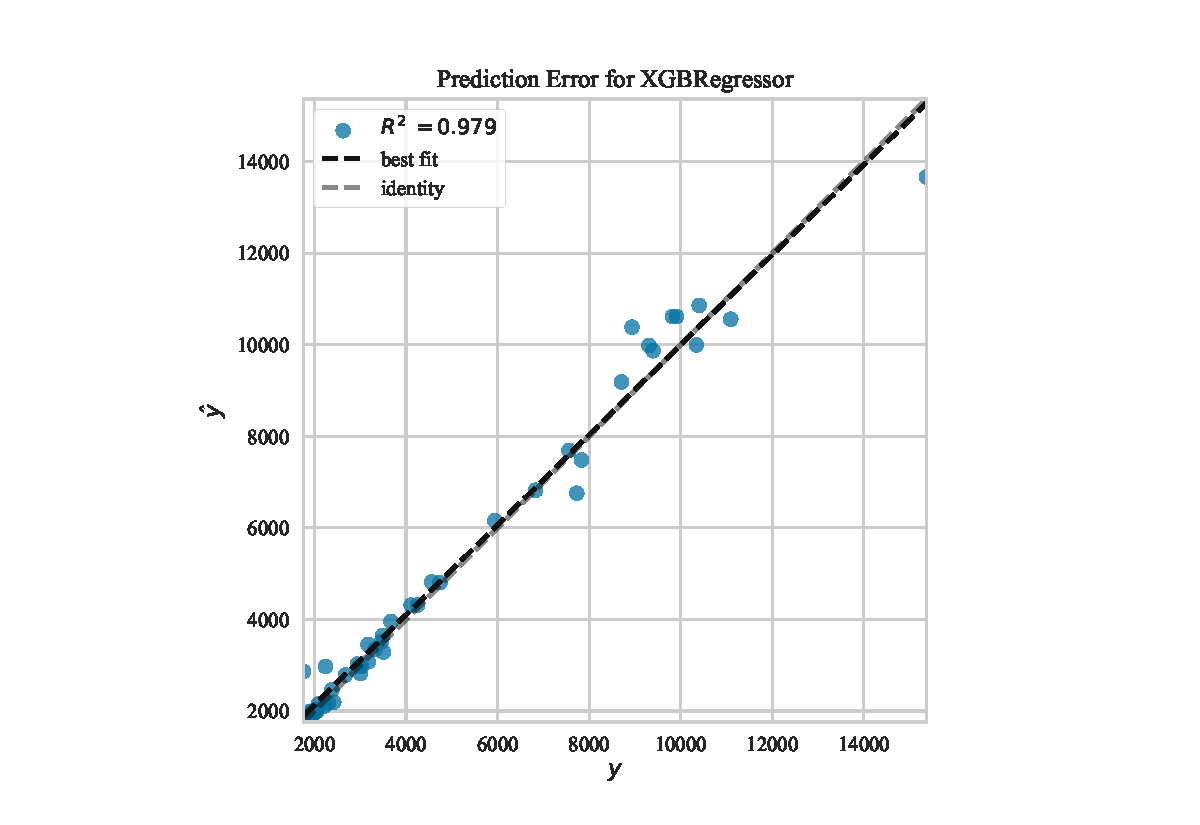
\includegraphics[width=1.0\linewidth]{XGBoost预测误差(困难人数).pdf}
			\caption{XGBoost预测误差-困难人数}
			\label{fig:XGBoost预测误差困难人数}
		\end{minipage}
	\end{figure}
	此外,我们还计算出模型的平均绝对误差(Mean Absolute Error,MAE)、均方误差(Mean Squared Error,MSE)、均方根误差(Root Mean Squared Error,RMSE),以及拟合优度(Goodness of Fit)即$R^2$,其具体计算方式如下:
	\begin{itemize}
		\item \textbf{平均绝对误差}
			\begin{equation}
			\mathrm{MAE}=\frac{1}{n}\sum_{i=1}^{n}\left|y_{i}-\hat{y}_{i}\right| \label{MAE}
			\end{equation}
		\item \textbf{均方误差}
			\begin{equation}
			\mathrm{MSE}=\frac{1}{n}\sum_{i=1}^{n}\left(y_{i}-\hat{y}_{i}\right)^{2} \label{MSE}
			\end{equation}
		\item \textbf{均方根误差}
			\begin{equation}
			\mathrm{RMSE}=\sqrt{\frac{1}{n}\sum_{i=1}^{n}\left(y_{i}-\hat{y}_{i}\right)^{2}} \label{RMSE}
			\end{equation}
		\item $\boldsymbol{R^2}$
			\begin{equation}
			R^{2}=\frac{\sum\limits_{i=1}^{n}\left(\hat{y}_{i}-\overline{y}\right)^{2}}{\sum\limits_{i=1}^{n}\left(y_{i}-\overline{y}\right)^{2}} \label{R2}
			\end{equation}
	\end{itemize}

	最终计算结果见\textcolor{blue}{\cref{tab:XGBoost预测结果}}。
\begin{table}[H]
	\centering
	\caption{XGBoost回归预测结果}
	\scalebox{0.95}{
	  \begin{tabular}{ccccc}
	  \toprule
	  \textbf{预测} & \textbf{MAE} & \textbf{MSE} & \textbf{RMSE} & $\boldsymbol{R^2}$ \\
	  \midrule
	  总人数   & 2586  & 29849352 & 5463  & 0.9957 \\
	  困难人数  & 97    & 38334 & 196   & 0.9959 \\
	  \bottomrule
	  \end{tabular}}
	\label{tab:XGBoost预测结果}
\end{table}
  
根据上述结果,我们可以发现XGBoost回归预测对于该数据集有较优表现,预测效果良好,在误差允许范围内。

现我们将对2023年5月15日报告情况进行预测,并且为使分析更具有一般性,我们给出在$95\,\%$的置信水平下的预测区间。但在上述分析中,我们发现对于每日报告的人数并不服从正态分布,这是由于我们选取Wordle从发布至今的每日人数情况进行分析,但游戏从发布至今存在增长、成熟、衰退与稳定的时期。根据\textcolor{blue}{\cref{fig:XGBoost预测结果总人数}}及\textcolor{blue}{\cref{fig:XGBoost预测结果困难人数}}所示结果,我们可以发现从2023年6月开始,Wordle的人数将会进入稳定期,对于该时期的数据我们有理由认为其每日报告的人数服从正态分布。因此我们可以利用\textcolor{blue}{\cref{tab:XGBoost预测结果}}中的均方根误差(RMSE)来计算预测区间,其计算方式如下:

记每日报告人数为$X$,则$X\sim N(\mu,\sigma^2)$,其中$\mu$为样本均值,这里由于处于稳定期,我们假设预测值近似为样本均值,$\sigma$为RMSE,则标准误差为
\begin{equation}
	\text{SE}=\frac{\sigma}{\sqrt{n}}=\frac{\text{RMSE}}{\sqrt{n}}
\end{equation}
其中$n$为样本总量。这里我们设定预测区间为$95\,\%$的置信水平,则有
\begin{equation}
	P(\mu-2\cdot\text{SE} < X < \mu+2\cdot\text{SE})=0.95
\end{equation}
因此$95\,\%$的置信区间为
\begin{equation}
	\left[\mu-2\sigma,\mu+2\sigma\right]
\end{equation}

通过上述分析,预测具体结果见\textcolor{blue}{\cref{tab:2023年5月15日报告情况预测}}。
\begin{table}[H]
	\centering
	\caption{2023年5月15日报告情况预测结果}
	\scalebox{0.95}{
	  \begin{tabular}{cccccc}
	  \toprule
	  \textbf{预测} & \textbf{预测值} & \textbf{RMSE} & \textbf{SE} & \textbf{区间下界} & \textbf{区间上界} \\
	  \midrule
	  总人数   & 18334 & 5463  & 251   & 17831  & 18352  \\
	  困难人数  & 1874  & 196   & 9     & 1856  & 1892  \\
	  \bottomrule
	  \end{tabular}}
	\label{tab:2023年5月15日报告情况预测}
\end{table}

因此,我们得到最终预测结果,即2023年5月15日的报告情况为:报告总人数为$\left[17831,18352\right]$人,选择困难模式游戏的人数为$\left[1856,1892\right]$人。
	\subsubsection{单词属性与玩家在游戏中的表现关系}
	
	\subsection{问题二模型的建立与求解}
	
	\subsection{问题三模型的建立与求解}
  
	\subsection{问题四}

	\subsection{问题五}

\section{模型的评价与推广}
	\subsection{模型的评价}
	\begin{itemize}
		\item \textbf{模型的优点}:
			\begin{enumerate}
				\item 
				\item 
			\end{enumerate}
		\item \textbf{模型的缺点及改进}:
			\begin{enumerate}
				\item 
				\item 
			\end{enumerate}
	\end{itemize}
	\subsection{模型的推广}
	
	\newpage
	\phantomsection
	\addcontentsline{toc}{section}{\textbf{参考文献}}
	\begin{spacing}{1.08}
	\begin{thebibliography}{99}
	\bibitem{pxgboost1}陈振宇,刘金波,李晨,季晓慧,李大鹏,黄运豪,狄方春,高兴宇,徐立中.基于LSTM与XGBoost组合模型的超短期电力负荷预测[J].电网技术,2020,44(02):614-620.DOI:10.13335/j.1000-3673.pst.2019.1566.

	\bibitem{pxgboost2}杨贵军,徐雪,赵富强.基于XGBoost算法的用户评分预测模型及应用[J].数据分析与知识发现,2019,3(01):118-126.

	\bibitem{pxgboost3}Tianqi Chen and Carlos Guestrin. 2016. XGBoost: A Scalable Tree Boosting System. In Proceedings of the 22nd ACM SIGKDD International Conference on Knowledge Discovery and Data Mining (KDD '16). Association for Computing Machinery, New York, NY, USA, 785–794. \url{https://doi.org/10.1145/2939672.2939785}.

	\end{thebibliography}
	\end{spacing}
	\newpage

	\phantomsection
	\addcontentsline{toc}{section}{\textbf{附\hspace{2pc}录}}

	% \appendix
	% \ctexset{section={format={\zihao{-4}\heiti\raggedright}}}
	\begin{center}
		\heiti\zihao{4} 附\hspace{2pc}录
	\end{center}

% \phantomsection
% \addcontentsline{toc}{subsection}{[A]图示}
	% \section*{[A]图示}
	\noindent{\heiti [A]图示}
	
\newpage
% \phantomsection
% \addcontentsline{toc}{subsection}{[B]支撑文件列表}
	% \section*{[B]支撑文件列表}
	\noindent{\heiti [B]支撑文件列表}
	~\\

	支撑文件列表如下(列表中不包含原始数据集以及中途产生的临时数据文件):

\begin{table}[H]
	\centering
	  \begin{tabular}{cc}
	  \toprule
	  \textbf{文件夹名} & \textbf{描述} \\
	  \midrule
	  html文件 & 包括所有解决问题的源程序运行结果 \\
	  ipynb文件 & 包括所有解决问题的源程序源代码 \\
	  py文件  & 包括所有解决问题的源程序输出python文件 \\
	  仿真结果  & 包括附件1的8次航班全时刻的飞行状态预警 \\
	  \bottomrule
	  \end{tabular}
\end{table}

	\noindent{\heiti [C]使用的软件、环境}
	~\\

	\textbf{C.1}:为解决该问题,我们所使用的主要软件有:
	\begin{itemize}
		\item TeX Live 2022
		\item Visual Studio Code 1.77.3
		\item WPS Office 2023春季更新(14036)
		\item Python 3.10.4
		\item Pycharm 2023.1 (Professional Edition)
	\end{itemize}

	\textbf{C.2}:Python环境下所用使用到的库及其版本如下:
\begin{table}[H]
	\centering
	\setlength{\aboverulesep}{0pt}
	\setlength{\belowrulesep}{0pt}
	\scalebox{0.85}{
	  \begin{tabular}{cc||cc}
	  \toprule
	  \textbf{库}     & \textbf{版本}    & \textbf{库}     & \textbf{版本} \\
	  \midrule
	  copy  & 内置库   & matplotlib & 3.5.2 \\
	  jupyter & 1.0.0 & numpy & 1.22.4+mkl \\
	  jupyter-client & 7.3.1 & openpyxl & 3.0.10 \\
	  jupyter-console & 6.4.3 & pandas & 1.4.2 \\
	  jupyter-contrib-core & 0.4.0 & pyecharts & 1.9.1 \\
	  jupyter-contrib-nbextensions & 0.5.1 & scikit-learn & 0.22.2 psot1 \\
	  jupyter-highlight-selected-word & 0.2.0 & sklearn & 0.0  \\
	  jupyterlab-pygments & 0.2.2 & snapshot\_phantomjs & 0.0.3 \\
	  jupyterlab-widgets & 1.1.0 & xgboost & 1.6.1 \\
	  jupyter-latex-envs & 1.4.6 & yellowbrick & 1.4 \\
	  jupyter-nbextensions-configurator & 0.5.0 &       &  \\
	  \bottomrule
	  \end{tabular}}
\end{table}
  
\newpage

\noindent{\heiti [D]问题解决源程序}

\textbf{D.1 航班1数据分析}

\newpage
\textbf{D.2 航班2数据分析}

\newpage
\textbf{D.3 航班3数据分析}

\end{document}